
	\section{Een eerste AEM applicatie}
	In de vorige hoofdstukken hebben we services voorzien die data op verscheidene manieren kunnen ophalen, het enige wat nog ontbreekt is een applicatie om deze te gebruiken. In dit deel gaan we onze eerste AEM applicatie bouwen en proberen we de verschillende manieren uit om deze applicatie van data te voorzien.
	\subsection{Een author lokaal draaien}
	Tijdens het ontwikkelen van een AEM-applicatie is het aangeraden om een lokale author te draaien. We kunnen deze omgeving gebruiken om onze geschreven componenten een eerste keer in actie te zien zonder deze op een remote server te moeten deployen. We hebben reeds gezien hoe we een author kunnen starten, om dit lokaal te doen volgen we hetzelfde proces.
	\subsection{Een Maven project aanmaken}
		Het gebruiken van een Maven project heeft verscheidene voordelen: we kunnen REST endpoints voorzien die men kan gebruiken om data naartoe te sturen (pagina's generen), business logica ontwikkelen in de vorm van Java-klassen en we kunnen het project beheren via git waardoor we met meerdere aan één component kunnen werken. Het handmatig aanmaken van zo'n project kan lastig zijn, gelukkig voor ons heeft Adobe een template project voorzien die we kunnen gebruiken.
		
	\begin{figure}[h!]
  		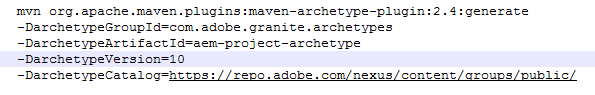
\includegraphics[width=\linewidth]{images/maven-archetype.PNG}
  		\caption{Maven commando.}
  		\label{fig:maven-archetype}
	\end{figure}

Wanneer we commando van Figuur \ref{fig:maven-archetype} uitvoeren (vereist Maven versie 3.3.1 of hoger) wordt ons gevraagd om enkele zaken te specificeren zoals de naam van onze website, de naam van onze modules en OSGi-bundels. Wanneer deze zijn ingevuld wordt het project aangemaakt en kunnen we aan de slag gaan.
	\subsection{Structuur van het Project}
	Wanneer we het project openen zien we dat de template voorzien is van meerdere modules die elk dezelfde prefix maar andere suffix hebben, we overlopen kort de belangrijkste. De core-module bevat onze Java-klassen: repositories,dto's, rest controllers, onze modellen, enz. De ui.apps-module bevat het frontend gedeelte: de HTML, CSS, JavaScript, templates, enz. De ui.content-module bevat onze effectieve website, wanneer we deze deployen worden alle pagina's vervangen door wat er zich in deze module bevindt. Als onze Maven profielen ongewijzigd zijn gebeurt dit samen met het deployen van de ui.apps-modulen (dus wanneer we onze componenten bundel uploaden). Vanzelfsprekend willen we niet bij elke deploy alle pagina's van onze website verwijderen dus splitsen we deze uit naar een ander profiel. Voor het coderen van componenten houden we ons voornamelijk bezig met de core en ui.apps-module.
	\subsection{Een component maken}
	
	\begin{wrapfigure}{l}{0.5\textwidth}
  		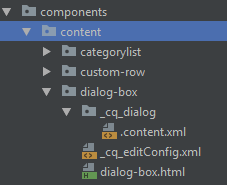
\includegraphics[width=0.5\textwidth]{images/component-pck-structure.PNG}
	\end{wrapfigure}
	Voor wie nog geen ervaring heeft met het aanmaken van componenten via een Maven project kan het moeilijk zijn om het doel van elk bestand te achterhalen, bijkomend is de documentatie schaars en vooral gericht op het werken met de author. In dit stuk gaan we een simpele component aanmaken en verklaren we wat waarvoor dient.
	\par
	Een component bestaat uit verschillende files gedefini\"erd onder een folder die de naam van de component draagt. Ter illustratie maken we een dialog-box component, als eerste maken we de folder aan. In deze folder defini\"eren we een "dialog-box.html" wat de structuur zal beschrijven. Als basis gebruiken we een Bootstrap panel waarbij we een titel en een tekst kunnen invullen. Vervolgens voegen we een "\_cq\_editConfig.xml" wat ons toelaat te bepalen hoe deze component gebruikt kan worden, enkele voorbeelden zijn: of deze via de author mag versleept worden, of de inhoud gewijzigd kan worden en op welke type pagina's deze component geplaatst kan worden. Als laatste hebben we een ".content.xml", hierin kunnen we specificeren wat er aan de component kan meegegeven worden wanneer deze op een pagina wordt gesleept. In ons voorbeeld voorzien we drie zaken: een titel, een tekst en de afmeting van de component.
	\begin{figure}[h!]
  		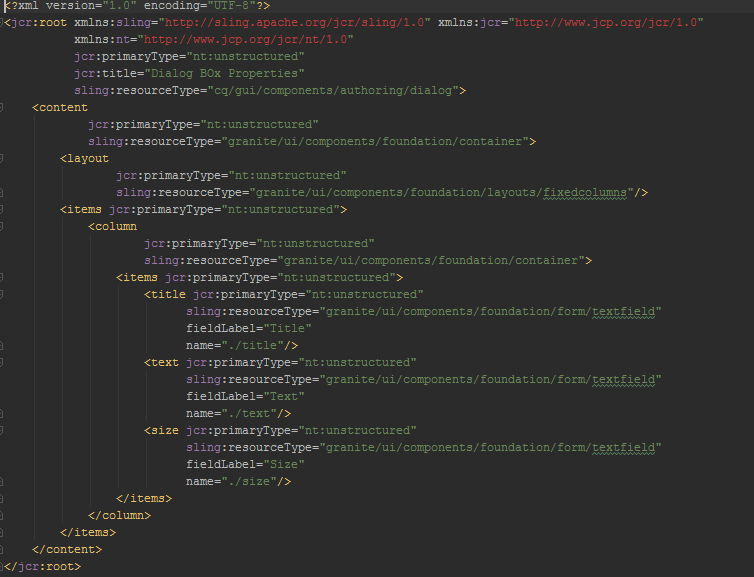
\includegraphics[width=\linewidth]{images/content-xml.PNG}
  		\caption{.content.xml}
  	\end{figure}
	\par
	We kunnen ook een Java-klasse voorzien waarop we de velden van de ".content.xml" kunnen injecteren. De Java klasse werkt als placeholder voor de velden van onze paginanode, als we een property 'jouw-tag:title' hebben voorzien we hiervoor een String en annoteren die met @Inject en @Named('jouw-tag:title'). Dit maakt het mogelijk om fallbacks in te bouwen alsook extra logica te voorzien, bv. een service gebruiken om data op te halen die we in onze HTML willen gebruiken.  
	\par
	Nu is het mogelijk om via Sightly onze klasse te koppelen aan onze HTML door het attribuut \textquotedbl data-sly-use.dialogBox="packagenaam-van-de-klasse.klasse-naam\textquotedbl{} in een tag toe te voegen. Het stuk na \textquotedbl data-sly-use.\textquotedbl{} definieert hoe we deze gaan aanspreken, in ons voorbeeld hebben we deze dialogBox genoemd. Nu kunnen we binnen de tags onze klasse gebruiken via volgende syntax: \${dialogBox.title}, gegeven er een getTitle() methode op onze Java-klasse staat.
	